% Copyright (C) 2015 Chen-Pang He <http://jdh8.org/>
%
% This file may be distributed and/or modified under
%
% 1. LaTeX Project Public License
% 2. GNU Public License
%
% See the files COPYING.* for more details.

\documentclass{Slideshow}

\begin{document}
\title[微積分演習課]{臺北醫學大學微積分演習課}
\maketitle

\section{關於}
\begin{frame}{關於我}
    \begin{columns}[onlytextwidth]
        \begin{column}{0.6\textwidth}
            \begin{itemize}
                \item \href{http://my2.tmu.edu.tw/b101100025}{B101100025}
                \item \href{https://www.facebook.com/jdh863}{臉書}
                \item \href{https://plus.google.com/+\%E4\%BD\%95\%E9\%9C\%87\%E9\%82\%A6-jdh8}{Google+}
                \item 0918-319823
                    \begin{itemize}
                        \item 真是充滿火藥味的號碼
                    \end{itemize}
            \end{itemize}
        \end{column}

        \begin{column}{0.4\textwidth}
            \begin{flushleft}
                \newlength{\stickerwidth}
                \setlength{\stickerwidth}{\columnwidth - 1em}
                
\includegraphics[width=\stickerwidth]{Introduction/sticker.jpg}
            \end{flushleft}
        \end{column}
    \end{columns}
\end{frame}

\begin{frame}{課程內容}
    以培養解題能力為目標。先通過考試,後培養邏輯思辨能力。

    \begin{itemize}
        \item \href{https://jdh8.github.io/calculus-slides/}{投影片}
        \item \href{http://jdh8.org/category/calculus-course/}{考古題、上課影片}
        \item 網頁教材(建構中)
            \begin{itemize}
                \item \href{http://jdh8.org/calculus/}{部落格頁面}
                \item \href{https://zh.wikibooks.org/wiki/\%E5\%BE\%AE\%E7\%A7\%AF\%E5\%88\%86\%E5\%AD\%A6}{維基教科書}
            \end{itemize}
    \end{itemize}
\end{frame}

\begin{frame}{Copyleft}
    本系列教材具有圖文創作與程式創作的性質,所以同時以下列條款釋出。

    \begin{description}
        \item[CC BY-SA] 適合圖文創作
        \item[GPL\scriptsize~v3+] 適合程式創作
    \end{description}

    Copyleft 允許閱聽人自由使用、複製、研究、修改著作,但必須以相同方式分享。

    \begin{figure}
        \href
            {https://commons.wikimedia.org/wiki/File:Copyleft.svg}
            {
\includegraphics[width=5em]{Introduction/Copyleft.pdf}}
    \end{figure}
\end{frame}

\section{集合與函數}
\begin{frame}{先備知識}
    \begin{figure}
        \href
            {https://commons.wikimedia.org/wiki/File:Japanese_Senbeis.jpg}
            {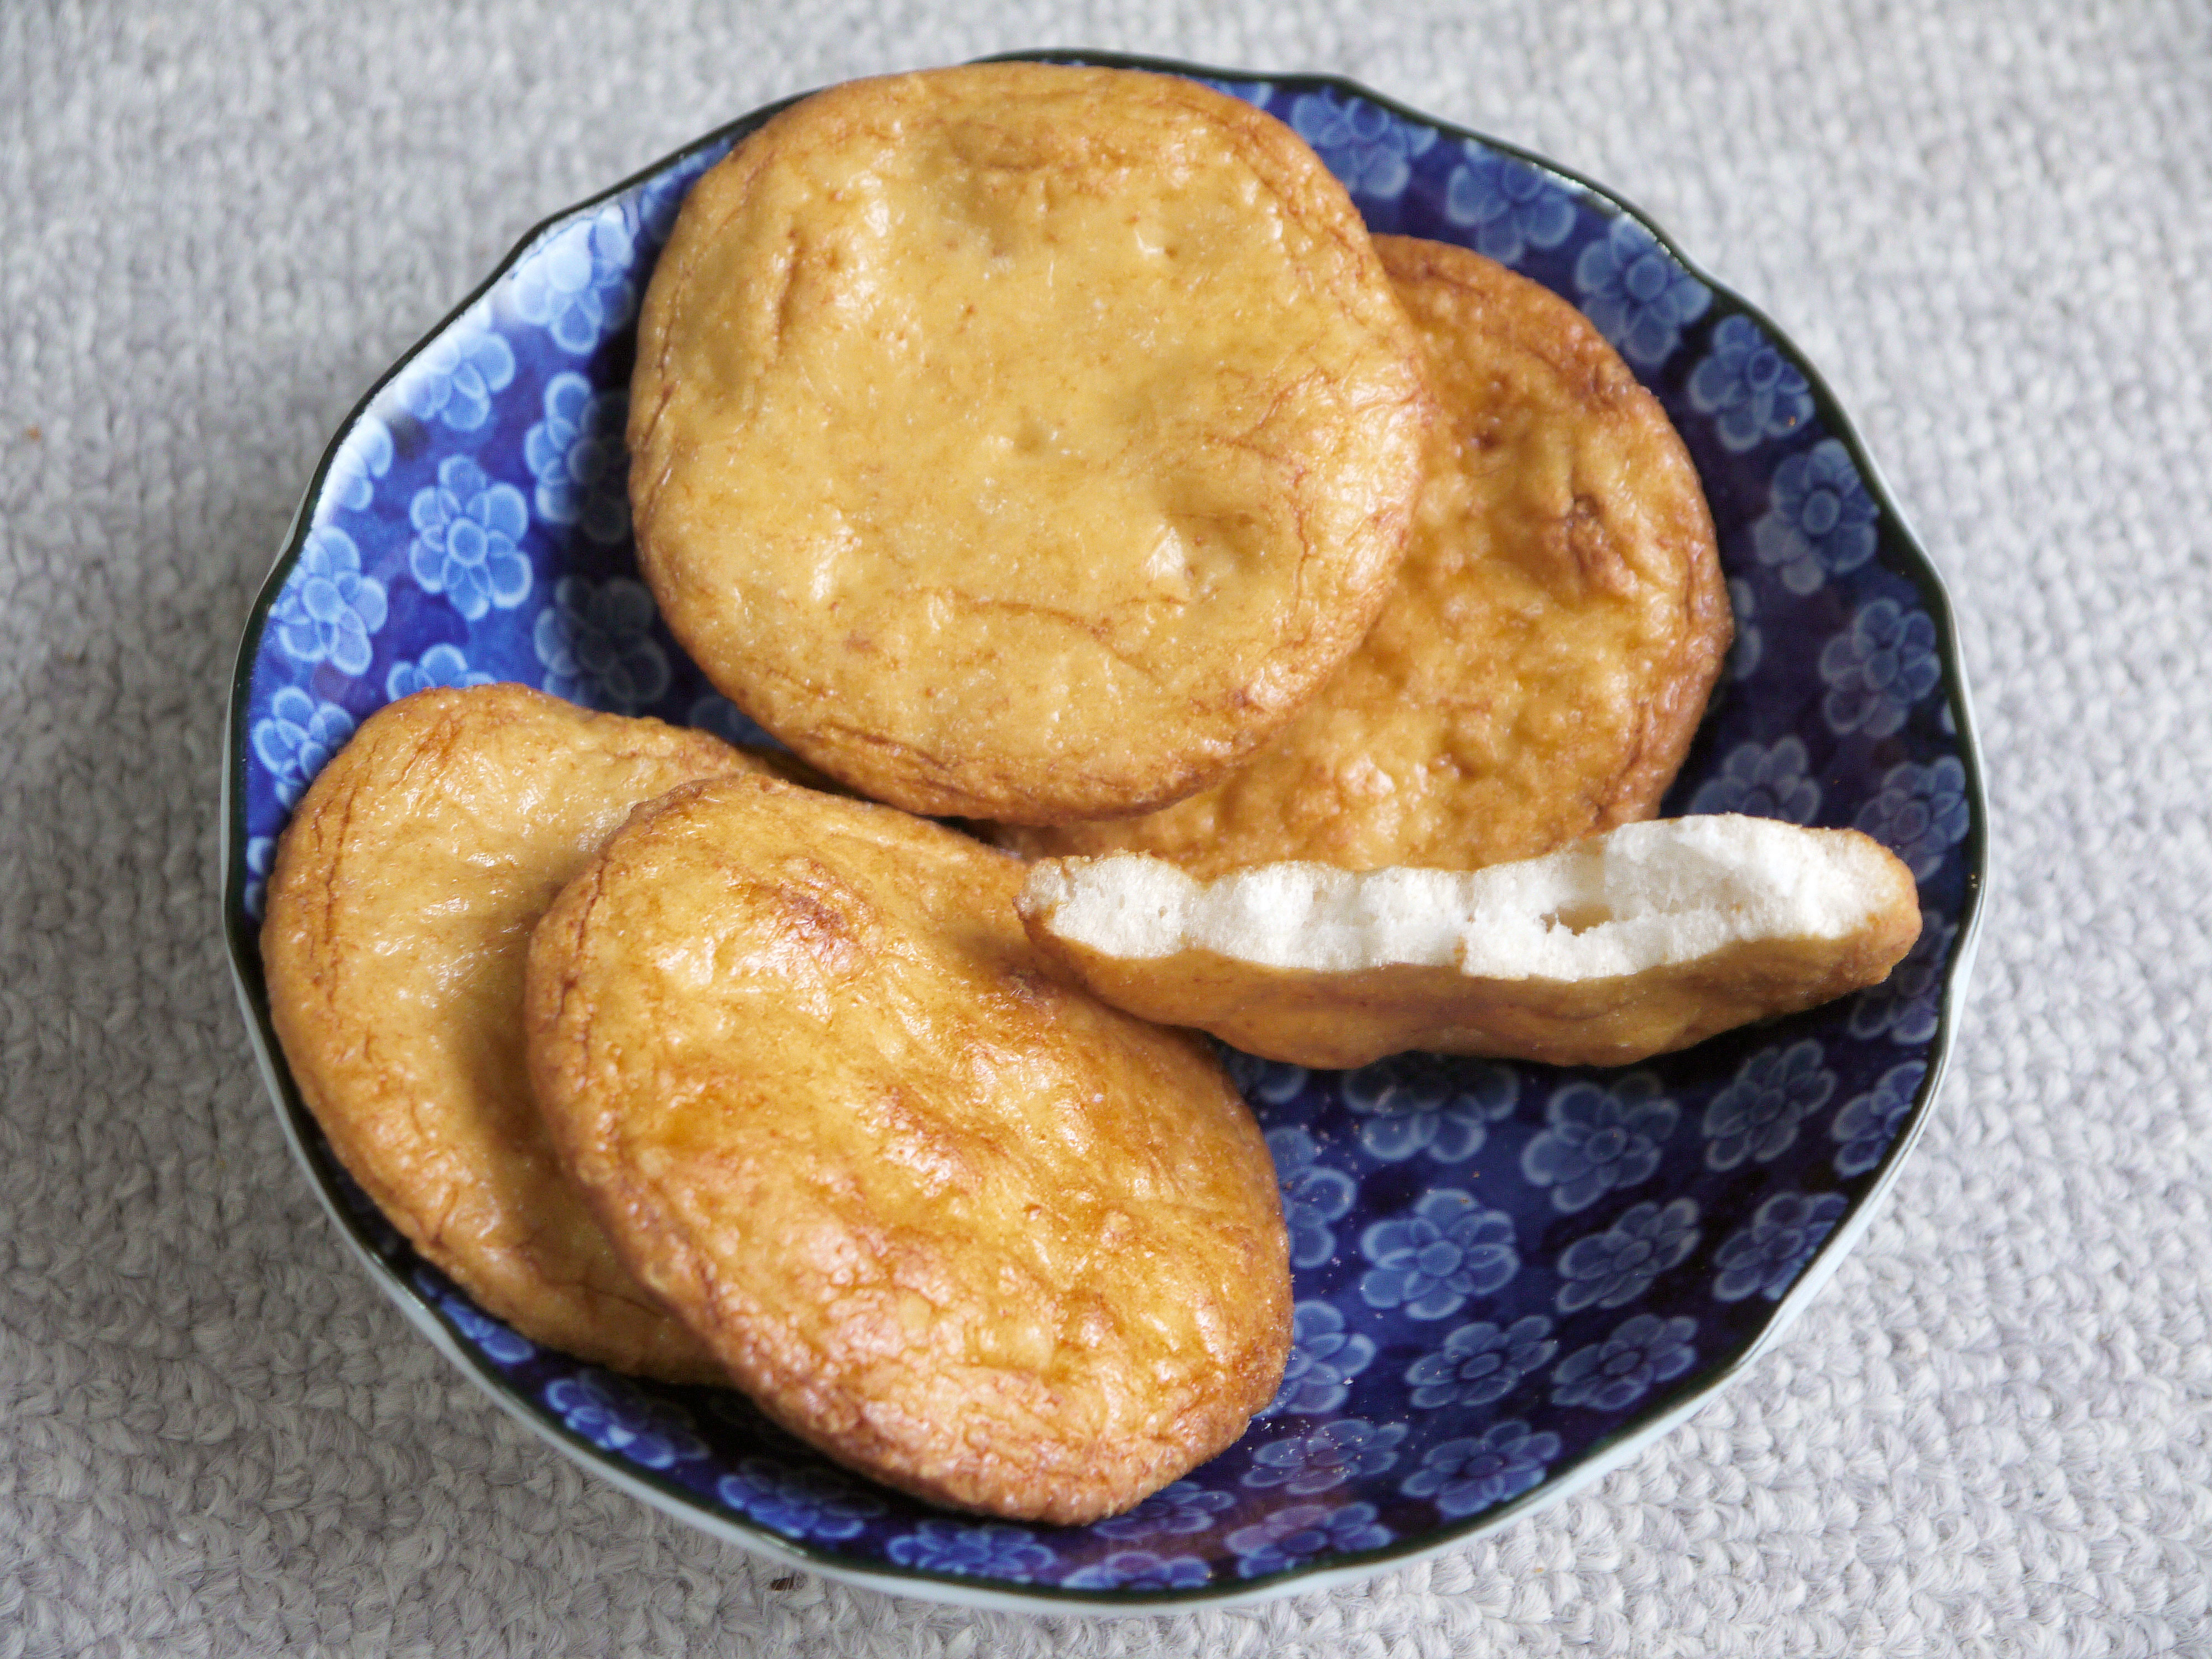
\includegraphics[width=\textheight]{Introduction/Japanese_Senbeis.jpg}}
        \caption{\href{https://ja.wikipedia.org/wiki/\%E7\%85\%8E\%E9\%A4\%85}{仙貝},由 DryPot 所攝}
    \end{figure}
\end{frame}

\begin{frame}{集合}
    當今所有數學實體都可視為集合。集合可以透過公理化集合論定義。
    \href{http://us.metamath.org/mpeuni/mmtheorems.html}{Metamath} 有精美範例。

    \begin{example}
        \[ \left( 3 + 5 \right) = 8 \]

        其中 + 是二元函數,也就是
        \[ +` \left\langle 3, 5 \right\rangle = 8 \]

        函數是關係的一種:
        \[ \left\langle \left\langle 3, 5 \right\rangle, 8 \right\rangle \in + \]
    \end{example}
\end{frame}
\end{document}
